\section{Introduction}\label{chp4:intro}

Early on in the history of VI investigations, it was discovered that many VI sites had significant temporal variation of indoor air contaminant concentration.
This variability presented a problem for all concerned, as it made it more difficult to assess the relevant human exposure at a site.
Of particular concern was the discovery that some sites were characterized by active and inactive periods.
This meant that it was possible for a VI investigation to give a false-positive result, further complicating things.\par

To address the growing concerns of temporal variability in VI, the EPA, together with Arizona State University (ASU), purchased a VI impacted building near Hill Air Force Base (AFB) in Utah.
(The primary contaminant source of concern here was the TCE contaminated groundwater.)
The purpose of this was to conduct a long-term high-resolution scientific inquiry, with which the rich dataset would reveal the nature of these temporal variabilities, and offer unprecedented insights into the VI phenomenon.
Another key objective was to assess the viability of the controlled pressure method (CPM) as an investigative tool (but more on that later).\par

The house in question, henceforth referred to as the ASU house, was outfitted a wide array of instrumentation to monitored a slew of factors deemed pertinent for VI, e.g. building pressurization, weather factors, air exchange rate, and much more.
Of most significance was the measuring of contaminant concentrations inside the building, but also in the soil-gas, and contaminated groundwater below.
Many soil-gas and groundwater probes were placed at different locations and depths - detailing how the contaminant was distributed throughout the soil and groundwater around the house.
Indoor air sampling also took place in different parts of the building.\par

The measurements, in particular indoor air contaminant concentration measurements, revealed what was perhaps one of the most significant temporal variabilities recorded at a VI site.
Figure \ref{fig:asu_indoor_concentration} shows this variability across the entire 3.5 years study period.
As can be seen, orders of magnitude of variability on both short- and long-term timescales were recorded at the site, causing even more concern about the nature of the variability.\par

\begin{figure}[htb!]
  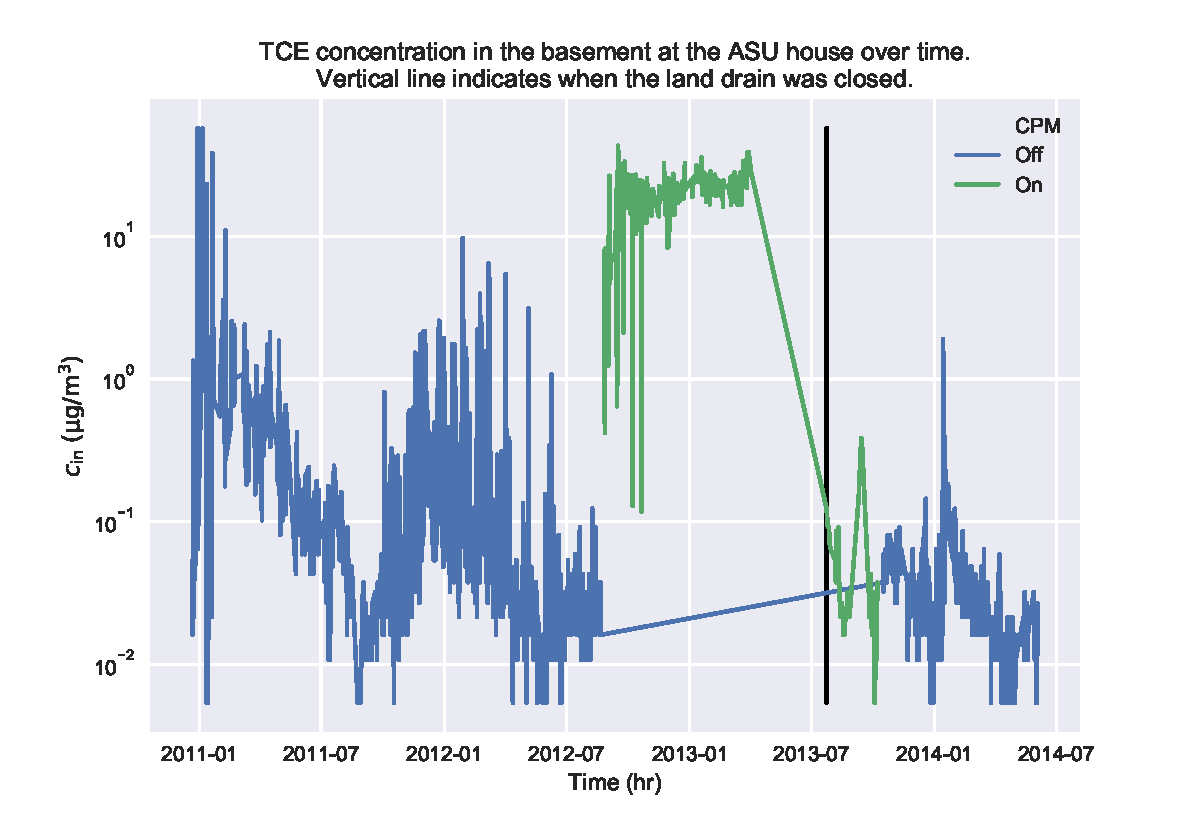
\includegraphics[width=\textwidth]{asu_indoor_concentration.pdf}
  \caption{The temporal variability of indoor air contaminant concentrations recorded at the ASU house. Measurements were taken in the basement. The periods were the CPM system was on and off are marked.}
  \label{fig:asu_indoor_concentration}
\end{figure}

The CPM was employed during the middle stages of the study, to see if and how the temporal variability would be reduced, this period is shown in Figure \ref{fig:asu_indoor_concentration}.
This had the desired effect and significantly reduced the variability, keeping the indoor air contaminant concentration relatively steady at the higher concentration observed during the "natural" or no-CPM phases.
While this was a success, it didn't explain why there was so much variability during the non-CPM periods.\par

It was not until the latter part of the CPM study phase that a land drain underneath the house was uncovered.
The purpose of this land drain was to drain any water from the gravel filled sub-slab into the sewer (which it was connected to).
The researchers dug out the land drain and fitted a valve on it, allowing them to turn it's influence on and off.\par

The land drain was first turned off during the end of CPM phase of the study, dramatically decreasing the indoor concentration, reaching concentrations that are more similar to the lower end of the concentrations during the natural period.
We can also see that the indoor concentrations never reached the same high levels during the subsequent natural period (after the CPM period) as there were before when the land drain was open.
This clearly shows the significant effect that the land drain had on the contaminant transport, during both natural and CPM periods, which is clearly shown in Figure \ref{fig:asu_concentration_boxplot}.\par

\begin{figure}[htb!]
  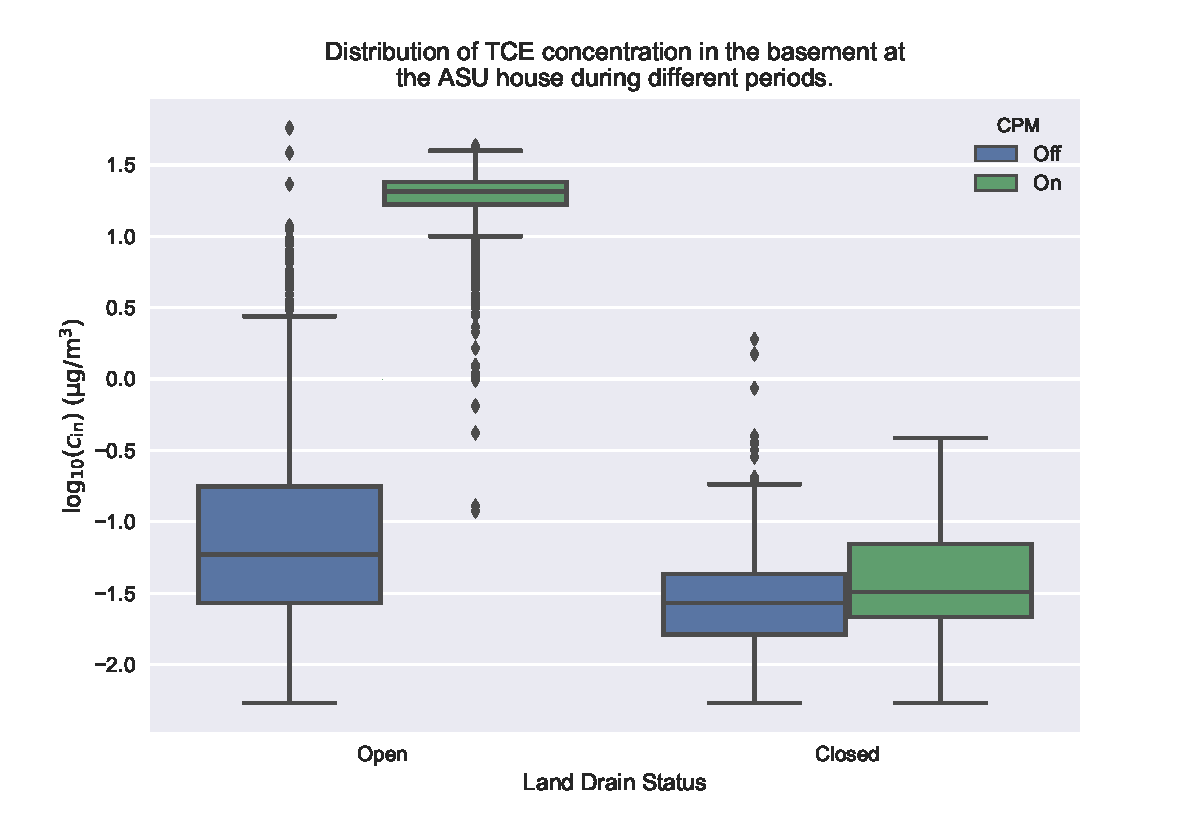
\includegraphics[width=\textwidth]{asu_boxplot_concentration.pdf}
  \caption{Boxplot showing the log-10 transformed TCE concentrations at the ASU house. The CPM and natural periods, and the period before and after the land drain was closed are considered separately. The box signifies the interquartile range (IQR) of values, with the central line representing the median value, and the top and bottom of the box are the 25th and 75th percentiles. The whiskers extend to 1.5 times the IQR. Markers indicate outlier data points that fall outside the whiskers.}
  \label{fig:asu_concentration_boxplot}
\end{figure}

The question then becomes, why did the land drain, hereafter referred to as simply a preferential pathway, so significantly change the nature of the VI site?
Figure \ref{fig:asu_concentration_boxplot} clearly shows that when the preferential pathway was open, CPM did what was expected and maximized the indoor concentration.
But after the preferential pathway was closed, CPM had a minimal effect on this, and the distributions of indoor concentration values are not so different from those during the post-CPM and post-preferential pathway period.\par

In the VI field, it is widely held that the building pressurization relative to the ambient outdoor is a key driver of contaminant entry into VI impacted building.
Since building pressurization fluctuations can occurs rapidly, this is a prime factor for investigating the transport dynamics of the preferential pathway.
Thus to examine the physical implications of such a preferential pathway we consider the relationship between the indoor air concentration and building pressurization, specifically indoor/outdoor pressure difference, for the periods when the preferential pathway was open and closed, the result of which is shown in Figure \ref{fig:asu_pressure_dependence}.\par

\begin{figure}[htb!]
  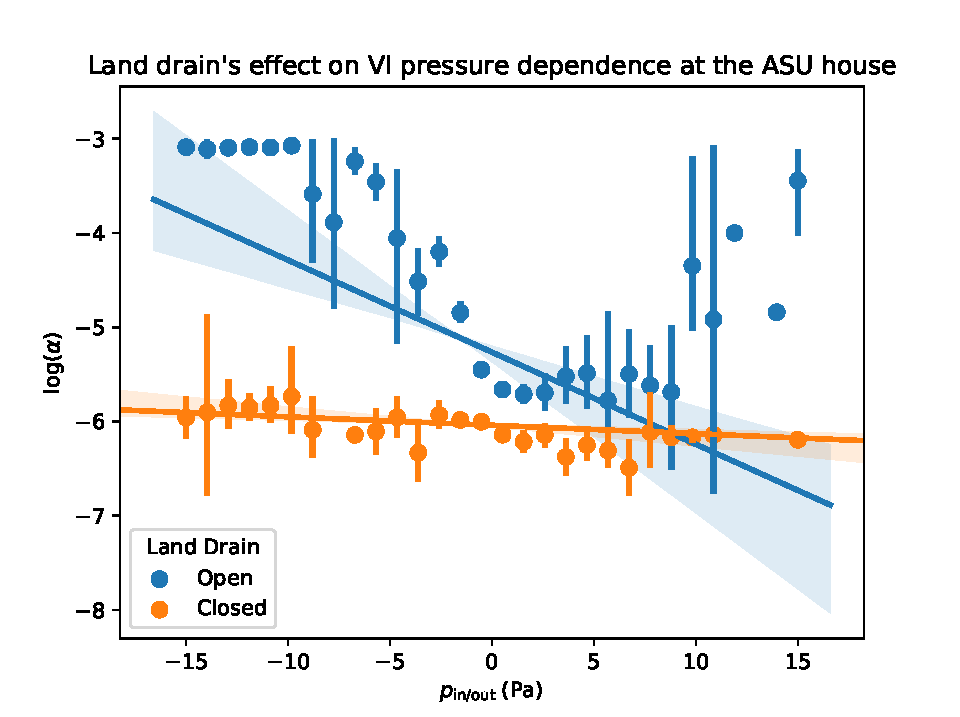
\includegraphics[width=\textwidth]{asu_pressure_dependence.pdf}
  \caption{Regression plot showing the indoor/outdoor pressure difference dependence on indoor air concentration. Here the indoor air concentration is normalized to the groundwater source concentration, i.e. attenuation factor, and log-10 transformed. Data is placed in evenly spaced (but not sized) bins. The bars indicate the 95\% confidence intervals.}
  \label{fig:asu_pressure_dependence}
\end{figure}

Based on this figure we see that the indoor air concentration has a much stronger correlation with building pressurization when the preferential pathway was open than it had when it was closed.
This suggests that the presence of the preferential pathway significantly enhanced the advective transport potential at the site.
However, we also see that the relationship between indoor air concentration and pressurization is not linear; a threefold increase in depressurization does not result in a threefold increase in indoor air concentration, but a much greater increase.
This indicates that the preferential pathway does not merely enhance the airflow, leading to large advective transport, but also increases the contaminant concentration.\par

Indeed, if we were to look at the indoor air concentration normalized to the near-foundation contaminant concentration (see Figure \ref{fig:asu_subslab_attenuation}) we can see that the attenuation is at times greater than unity.
% Which proves that hte subsurface contaminant concentration was much higher during LD open and has huge spatial variability.

\begin{figure}[htb!]
  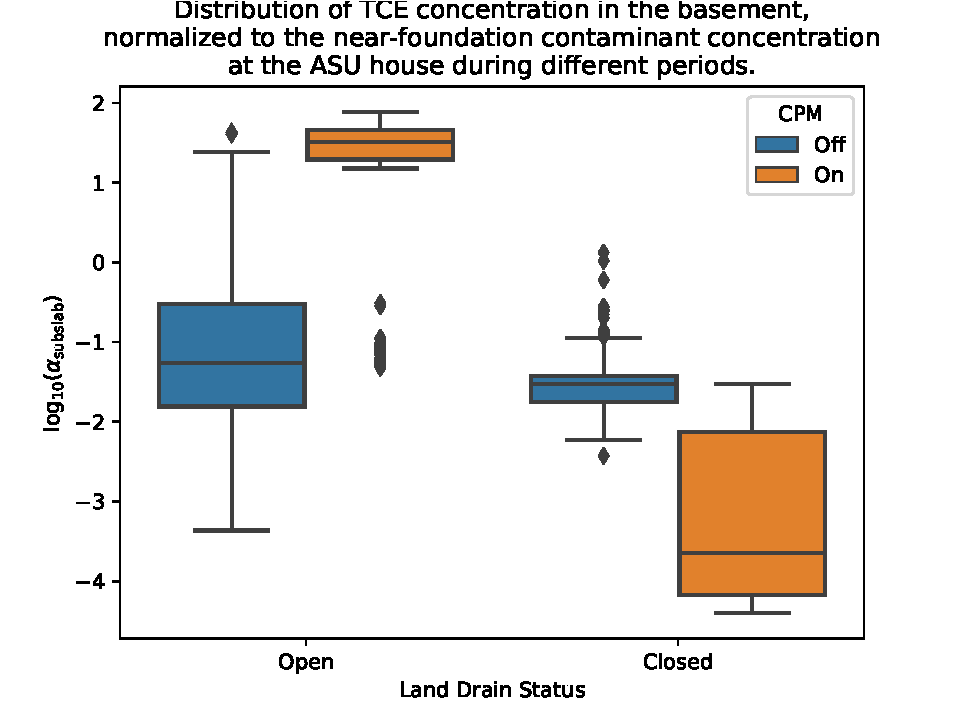
\includegraphics[width=\textwidth]{asu_subslab_attenuation.pdf}
  \caption{TBD}
  \label{fig:asu_subslab_attenuation}
\end{figure}
